\section{Kvantevandringer}

\subsection{Grover's algoritme og metoden av amplitude amplifikasjon}

    Grover's algoritme løser problemet med ustrukturert søk, og teknikken amplitude amplifikasjon som den bruker er av stor interesse. Problemet går som følger: Tenk at man er gitt en bistring med $N=2^n$ bits, hvor $t$ bits er satt til 1. Finn minst 1 bit som har verdi 1. Dette problemet kan åpenbart løses i "worstcase"\ lineær tid med konstant minne ved å randomisert iterere gjennom alle bitene og sjekke om de er 1 eller 0. Om den er 1 kan man terminere programmet, og returnere den posisjon som ga 1. Grover's algoritme har en kvadratisk hastighetsøkning på dette problemet, og man kan dermed løse det i worst case kvadratisk tid.

    For å beskrive problemet med et fysisk kvantesystem trenger vi å oversette problemet først. La $(b_k)_N$ være bitstringen med lengde N, definer så orakelet $\mathcal{O}_{(b_k)_N}:\mathbb{C}^{2^n} \otimes \mathbb{C}^2 \rightarrow \mathbb{C}^{2^n} \otimes \mathbb{C}^2$ til å merke målbiten hvis registerbiten var en løsning. Dette vil si at hvis $\mathcal{O}_{(b_k)_N}(|r\rangle\otimes |0\rangle) = |r\rangle\otimes |1\rangle$ så følger det at $b_r = 1$. For å fullføre Grover's algoritme trenger man matrisen $R$ som flipper fortegnet til registeret hvis den ikke er tilstanden $|0\rangle^{\otimes n}$.
    \begin{center}
        \begin{math}
            R = \begin{pmatrix}
                1 & 0 & ... \\
                0 & -1 & ... \\
                \vdots & \vdots & \ddots
            \end{pmatrix}
            %= 2|0\rangle\langle 0| - I
        \end{math}
    \end{center}

    En Grover iterate $\mathcal{G}$ er definert som 
    \begin{align*}
        \mathcal{G}=H^{\otimes n}RH^{\otimes n}\mathcal{O}_{(b_k)_N, \pm}.
    \end{align*}
    
    Gorver's algoritme er komposisjonen av operatorene $G = M\mathcal{G}^k\circ H^{\otimes n}$, hvor $M$ er en projektiv måling, og $k$ er en konstant. Man skal da kunne fastslå med en høy sannsynlighet at målingen gir deg posisjonen til en bit i $(b_k)_N$ som er $1$. For å finne denne $k$-en som man bruker for å kjøre algoritmen trenger vi å se på metoden av amplitude amplifikasjon.

    Definer tre tilstander hvor $t$ er antall $1$-ere i $(b_r)_N$ 
    \begin{align*}
        u & = H^{\otimes n}|0\rangle^{\otimes n}\\
        G & = \frac{1}{\sqrt{t}}\Sigma_{|r\rangle \mid b_r = 1}|r\rangle\\ 
        B & = \frac{1}{\sqrt{N-t}}\Sigma_{|r\rangle\mid b_r = 0}|r\rangle
    \end{align*}. 

    \begin{figure}
        \caption{Grover's algoritme}
        \begin{center}
            \begin{subfigure}[b]{0.46\textwidth}
                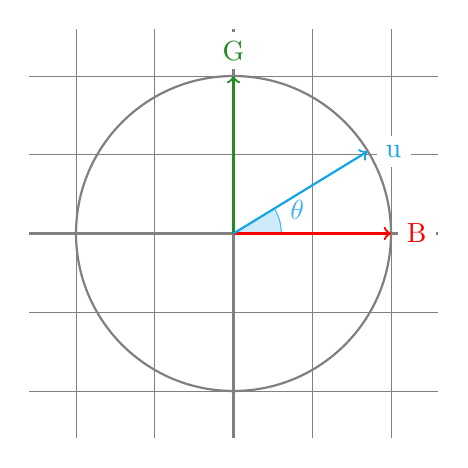
\begin{tikzpicture}[scale=2]
                    \draw[step=.5,gray,very thin] (-1.3,-1.3) grid (1.3,1.3);
                    \draw[gray, thick] (0,0) circle (1);
                    \draw[gray, thick] (1.3, 0) -- (-1.3, 0);
                    \draw[gray, thick] (0, 1.3) -- (0, -1.3);
                    \draw[ForestGreen, thick, ->] (0,0) -- (0, 1) node[above=2pt, fill=white] {G};
                    \draw[Cerulean!80!White, thick] (0.3, 0) arc (0:30:0.3) node[right=2pt] {$\theta$};
                    \fill[Cerulean!20!White] (0,0) -- (0.3, 0) arc (0:30:0.3) -- (0,0);
                    \draw[Red, thick, ->] (0,0) -- (1,0) node[right=2pt, fill=white] {B};
                    \draw[Cerulean, thick, ->] (0,0) -- (0.85,0.52) node[right=3pt, fill=white] {u};
                \end{tikzpicture}
                \caption{Initiell tilstand}
                \label{fig:Grover init}
            \end{subfigure}
            \begin{subfigure}[b]{0.46\textwidth}
                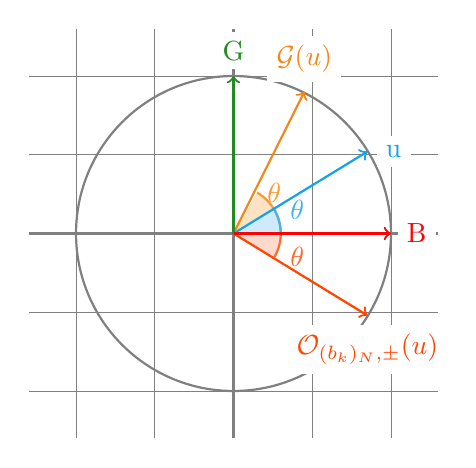
\begin{tikzpicture}[scale=2]
                    \draw[step=.5,gray,very thin] (-1.3,-1.3) grid (1.3,1.3);
                    \draw[gray, thick] (0,0) circle (1);
                    \draw[gray, thick] (1.3, 0) -- (-1.3, 0);
                    \draw[gray, thick] (0, 1.3) -- (0, -1.3);
                    \fill[BurntOrange!20!White] (0,0) -- (0.3, 0) arc (0:60:0.3) -- (0,0);
                    \fill[Cerulean!20!White] (0,0) -- (0.3, 0) arc (0:30:0.3) -- (0,0);
                    \fill[OrangeRed!20!White] (0,0) -- (0.3, 0) arc (0:-30:0.3) -- (0,0);
                    \draw[BurntOrange!80!White, thick] (0.3, 0) arc (0:60:0.3) node[right=0pt] {$\theta$};
                    \draw[Cerulean!80!White, thick] (0.3, 0) arc (0:30:0.3) node[right=2pt] {$\theta$};
                    \draw[OrangeRed!80!White, thick] (0.3, 0) arc (0:-30:0.3) node[right=2pt] {$\theta$};
                    \draw[Cerulean, thick, ->] (0,0) -- (0.85,0.52) node[right=3pt, fill=white] {u};
                    \draw[BurntOrange, thick, ->] (0,0) -- (0.45,0.9) node[above=3.2pt, fill=white] {$\mathcal{G}(u)$};
                    \draw[OrangeRed, thick, ->] (0,0) -- (0.85,-0.52) node[below=3pt, fill=white] {$\mathcal{O}_{(b_k)_N,\pm}(u)$};
                    \draw[ForestGreen, thick, ->] (0,0) -- (0, 1) node[above=2pt, fill=white] {G};
                    \draw[Red, thick, ->] (0,0) -- (1,0) node[right=2pt, fill=white] {B};
                \end{tikzpicture}
                \caption{En Grover iteration}
                \label{fig:Grover en}
            \end{subfigure}
        \end{center}
    \end{figure}
    
    Man kan se at $G$ (Good) og $B$ (Bad) vektorene er ortogonale, ettersom de er en sum av ortogonale vektorerer. I det 2 dimensjonale underrommet av $\mathbb{C}^{2^n}$ utspent av $G$ og $B$, finner man vektoren $u$.
    \begin{align*}
        u & = \frac{1}{\sqrt{N}}\Sigma_{|r\rangle}|r\rangle = \frac{\sqrt{t}}{\sqrt{N}}G + \frac{\sqrt{N-t}}{\sqrt{N}}B \\
        & = \sin\circ\arcsin(\frac{\sqrt{t}}{\sqrt{N}})G+\cos\circ\arcsin(\frac{\sqrt{t}}{\sqrt{N}})B \\
        & = \sin(\theta)G+\cos(\theta)B
    \end{align*}
    Her er $\theta = \arcsin(\frac{\sqrt{t}}{\sqrt{N}})$. Vi ønsker nå å manipulere tilstanden til $u$ i underrommet utspent av $G$ og $B$ for å maksimere $\sin(\theta)$. Dette vil maksimere sannsynligheten for at algoritmen avslutter i en tilstand hvor man har maksimal sjanse for å måle en qubit som er merket. La $\alpha:\mathbb{R}$ være en vinkel og $T = \sin(\alpha)G+\cos(\alpha)B$ være en tilstand. For å se hva orakelet gjør med $T$ kan vi se på hva den gjør med $G$ og $B$. 
    \begin{align*}
        & \mathcal{O}_{(b_k)_N, \pm}(B) = B \\
        & \mathcal{O}_{(b_k)_N, \pm}(G) = -G \\
        \implies & \mathcal{O}_{(b_k)_N,\pm}(T)=-\sin(\alpha)G+\cos(\alpha)B = \sin(-\alpha)G+\cos(-\alpha)B
    \end{align*}

    Operatoren $R$ har en annen beskrivelse som en refleksjon om en enhetsvektor.
    \begin{align*}
        R = 2|0\rangle^{\otimes n}\langle0|^{\otimes n} - I
    \end{align*}
    Det følger at den andre komponenten i en Grover's iterate er en refleksjon om tilstanden $u$.
    \begin{align*}
        & H^{\otimes n}RH^{\otimes n} \\ 
        & = H^{\otimes n}(2|0\rangle^{\otimes n}\langle0|^{\otimes n} -I)H^{\otimes n} \\ 
        & = 2H^{\otimes n}|0\rangle^{\otimes n}\langle0|^{\otimes n}H^{\otimes n} - H^{\otimes n}H^{\otimes n} \\ 
        & = 2uu^* - I
    \end{align*}
    En Grover's iterate kan derfor også bli betegnet som $\mathcal{G}=(2uu^*-I)\mathcal{O}_{(b_k)_N,\pm}$. Dette gjør at vi kan observere hva tilstanden til T er etter å anvende $H^{\otimes n}RH^{\otimes n}$ operatoren, og vi kan se hva Grover's iterate $k$ ganger gjør.
    \begin{align*}
        & H^{\otimes n}RH^{\otimes n}(T)=\sin(-\alpha + 2\theta)G+\cos(-\alpha + 2\theta)B \\
        \implies & \mathcal{G}^k(T)=\sin(\alpha+2k\theta)G+\cos(\alpha+2k\theta)B
    \end{align*} 
    Hvis man initialiserer $\alpha = \theta$ vil $k$ Grover's iterate gi
    \begin{align*}
        \mathcal{G}^k(T)=\sin((1+2k)\theta)G+\cos((1+2k)\theta)B.
    \end{align*}
    En naiv $k$ for når man skal stoppe Grover's algoritme er den tilstanden som er nærmest $G$ først.
    \begin{align*}
        & \sin((2k'+1)\theta) =1 \\
        \implies & (2k'+1)\theta = \frac{\pi}{2} \\
        \implies & k \approx \frac{\pi}{4\theta} - \frac{1}{2}=\lfloor\sfrac{\pi}{4\arcsin(\sqrt{\frac{t}{N}})}\rfloor.
    \end{align*}

    Denne verdien av $k$ vil gi sannsynligheten for å treffe et merket element 
    \begin{align*}
        p = \sin((1+2k)\theta) = \sin((1+\lfloor\sfrac{\pi}{2\arcsin(\sqrt{\frac{t}{N}})}\rfloor)\arcsin(\sqrt{\frac{t}{N}}))
    \end{align*}

    \subsubsection*{Sannsynlighet amplifikasjon og Amplitude amplifikasjon}

        Metoden av sannsynlighet amplifikasjon opererer på klassen av klassiske Monte Carlo algoritmer. En Monte Carlo algoritme er definert ved at den alltid returnerer et svar etter en endelig forhåndsbestemt tidsbegrensing, men svaret kan være feil. La $p$ være sannsynligheten for at algoritmen returnerer det riktige svaret innen $O(f(n))$. Sannsynlighets amplifikasjons algoritmen virker ved å kjøre algoritmen flere ganger, og dermed øker sjansen for at det riktige svaret har blitt avgitt. Hvis vi kjører algoritmen $n$ ganger så er sjansen for at minst et riktig svar har blitt gitt $1-(1-p)^n$. Gitt at $p\ll n$, så er sannsynligheten tilnærmet $1-(1-p)^n\approx np$. Ved å kjøre algoritmen $\sfrac{1}{p}$ ganger vil være en god tilnærming for å maksimere sannsynligheten for at det riktige svaret har blitt avgitt med kjøretid $O(\sfrac{f(n)}{p})$.
        
        Amplitude amplifikasjons algoritmen, bruker den samme ideen for å forbedre en kvantealgoritme, men ved å ikke bruke målinger så kan kjøretiden forbedres til $O(\sfrac{f(n)}{\sqrt{p}})$. Anta at det finnes en kvantealgoritme $A:\mathbb{C}nBits\rightarrow\mathbb{C}nBits$ som finner en tilstand som er merket. Funksjonen $f:nBits\rightarrow 1Bits$, bestemmer om et element er merket eller ikke. La $p$ være sannsynligheten for at $\psi = A\ket{n}$ er et merket element, hvor $\ket{n}$ er den beste initielle tilstanden til algoritmen $A$. Amplitude amplifikasjon virker ved å definere en ny operator
        \begin{align*}
            U = (2\psi\cdot\psi^*-I)\mathcal{O}_{f,\pm}.
        \end{align*}
        Her er $\mathcal{O}_{f,\pm}$ være faseoraklet definert utifra funksjonen $f$. Ved å kjøre operatoren $U$ $t=\lfloor\sfrac{\pi}{4\sqrt{p}}\rfloor$ ganger sannsynligheten mot $1$ for at utfallet av at algoritmen gir en merket bitstring. Analysen av denne algoritmen er nesten identisk som analysen av Grover's algoritme, for en fullstendig analyse referer jeg til \cite{portugal_2019}.

\subsection{Kvantevandringer basert på kvantemyntkast}

    Kvantevandringer prøver å ta ideen til Grover's algoritme for søk og å generalisere den til andre datatyper, som grafer. For å gjøre denne generaliseringen deler vi opp problemet inn i traversering og oppdagelse. Det er mange metoder for å traversere over grafer, og her er det noen viktige klasser med grafer som vi vil studere.

    % Tenker det kan være greit å forklare ideen med coin-shift prosessen her

    % Selve kvantevandringene kan sees på å være inspirert av de klassiske tilfeldig vandringsalgoritmene. For å illustrere et eksempel så kan man anta at man har en $d$-regulær graf, med $n$ noder. En nabomatrise $M$ for en slik graf vil være en $n\times n$-matrise hvor $d$ innlegg langs hver kolonne er $1$, som representerer dens nabo og resten er $0$. En sannsynlighetsmatrise $P=\frac{1}{d}M$ vil nå være en sannsynlighet for at hvis man står på node $v$, som har tilhørende kolonne $v$ i $P$, vil sannsynlighet for å dra til node $u$ være innlegget i den $u$-te raden i kolonne $v$ i $P$. Gitt en starttilstand som en vektor med $n$-dimensjoner, vil $P$ virke på denne vektoren og vise de mulige sannsynlighetene for hvor man kan flytte seg etter et steg. På denne måten vil $P$ danne en Markov kjede for den tilfeldige vandringen langs grafen.

    For å illustrere hvordan kvantevandring kan virke, starter vi med å se på en klassisk tilfeldig vandring. Se for deg at det er en vandrer som vandrer gjennom en skog med forgreninger. Når vandreren møter på en forgrening kaster de en mynt for å velge hvilken retning de går. En slik vandring vil være et eksempel på en rettet tilfeldig vandring over et binærtre. Denne ideen kan man gjøre om til en kvante vandringsalgoritme ved at man gjør om vandreren til en kvantepartikkel, med en kvantemynt som kan være i superposisjon av 2 forskjellige tilstander. Partikkelen vandrer gjennom skogen avhengig av tilstanden til mynten, akkurat som den klassiske vandreren. Dette tillater partikkelen til å flytte seg gjennom skogen som en superposisjon av forskjellige muligheter. Det vil først være når vi måler partikkelen sin posisjon at vi vil få vite hvor den er, og hvilke utfall mynten har gitt.

    For å være mer presis kan man tilegne to Hilbertrom til en slik kvantevandringsalgoritme. $\mathcal{H}_V$ representerer posisjonene til vandreren, og $\mathcal{H}_C$ representerer utfallene av kvantemyntkastet. Et kvantesteg defineres som komposisjonen av to operatorer $U=S(I\otimes C)$, en myntkast operator $C:\mathcal{H}_C\rightarrow\mathcal{H}_C$ som kaster mynten og en forflyttings operator (skift operater) $S:\mathcal{H}_V\otimes\mathcal{H}_C\rightarrow\mathcal{H}_V\otimes\mathcal{H}_C$ som leser av myntkastet og forflytter seg henholdsvis. En kvantevandring vil være en algoritme som $MU^kT$, hvor $M$ er en måling, $U$ er et kvantesteg og $T$ er en operator som setter systemet i starttilstanden. Dette er det som vi kaller for en myntbasert kvantevandringsalgoritme og er den formen for vandring som er standarisert i litteraturen.

    \subsubsection*{$d$-regulære grafer}

        Den første kvantevandringsmetoden som vi skal se på er vandring over $d$-regulære grafer, den kalles for \emph{position-coin notation}. For at denne metoden skal virke krever vi tillegg at det maksimale kantkromatiske tallet er det samme som $d$. Hvis man i tillegg ikke tillater at grafen har noen løkker vil spektraldekomposisjonen til algoritmen bli simplere.

        La $G=(V,E)$ være en $d$-regulær graf slik at det maksimale kantkromatiske tallet også er $d$. Siden kantene i grafen kan fargelegges med $d$ forskjellige farger, så kan vi separere grafen i $d$ forskjellige undergrafer. I hver undergraf er en node koblet til nøyaktig en annen node. La $\mathcal{H}_V = \mathbb{C}V$ være det frie Hilbertrommet over nodene og $\mathcal{H}_C = \mathbb{C}^d$ være myntrommet. Vi definerer forflyttingsoperatoren $S$ på følgende måte: La $f$ være en farge og $v:V$ en node. Assosiert med denne noden og fargen finnes det en unik node $v':V$, slik at det er en kant $(v,v'):E$ som har fargen $f$. 
        \begin{align*}
            S(v\otimes f)=v'\otimes f 
        \end{align*}
        Denne operatoren kalles for \emph{flip-flop operatoren}. En egenskap ved denne operaatoren som er enkel å bemerke er at $S^2 = I$, hvilket som gjør at den er hermitisk. 
        
        Myntoperatoren $C$ kan velges litt mer vilkårlig, men det er noen mynter som er bedre enn andre. En ønskelig egenskap fra mynten er at den er uniformt fordelt. Det kan finnes tilfeller hvor det er interessant å se på mynter som er vektet slik at en farge er vektet mer enn andre. Forskjellige normale valg av myntoperatorer kommer vi tilbake til senere.

        Et kvantesteg langs denne grafen kan man nå definere som $U=S(I\otimes C)$. Vi bemerker oss at egenskapen som lar oss bruke $I\otimes C$ er at grafen er $d$-regulær. Hvis grafen ikke hadde hatt denne egenskapen, men heller at den maksimale graden var lik det maksimale kantkromatiske tallet kan man fremdeles bruke det samme prinsippet. Siden vi ikke lengre kan være sikre på at alle noder har $d$ tilstøtende farger, så må man ha en mynt for hver node som tilordner ny farge langs den noden.

        \begin{figure}
            \caption{$4$-regulær graf}
            \begin{center}
                \begin{tikzpicture}[thick, main/.style = {draw, circle}]
                    \node[main] (1) at (0,0) {0};
                    \node[main] (2) at (1,0) {1};
                    \node[main] (3) at (1.71, 0.71) {2};
                    \node[main] (4) at (1.71, 1.71) {3};
                    \node[main] (5) at (1, 2.42) {4};
                    \node[main] (6) at (0, 2.42) {5};
                    \node[main] (7) at (-0.71, 1.71) {6};
                    \node[main] (8) at (-0.71, 0.71) {7};
                    \graph {
                        (1) --[color=red] (2) --[color=ProcessBlue] (3) --[color=red] (4) --[color=ProcessBlue] (5) --[color=red] (6) --[color=ProcessBlue] (7) --[color=red] (8) --[color=ProcessBlue] (1) --[color=LimeGreen] (4) --[color=magenta] (7) --[color=LimeGreen] (2) --[color=magenta] (5) --[color=LimeGreen] (8) --[color=magenta] (3) --[color=LimeGreen] (6) --[color=magenta] (1);
                    };
                \end{tikzpicture}
            \end{center}
            \begin{center}
                \subcaption*{Fargepartisjon av grafen}
                \begin{tcolorbox}
                    \begin{subfigure}{0.2451065\textwidth}
                        \begin{tikzpicture}[thick, main/.style= {draw, circle}, scale=0.75]
                            \node[main] (1) at (0,0) {};
                            \node[main] (2) at (1,0) {};
                            \node[main] (3) at (1.71, 0.71) {};
                            \node[main] (4) at (1.71, 1.71) {};
                            \node[main] (5) at (1, 2.42) {};
                            \node[main] (6) at (0, 2.42) {};
                            \node[main] (7) at (-0.71, 1.71) {};
                            \node[main] (8) at (-0.71, 0.71) {};

                            \graph {
                                (1) --[color=red] (2);
                                (3) --[color=red] (4);
                                (5) --[color=red] (6);
                                (7) --[color=red] (8);
                                };
                        \end{tikzpicture}
                        \subcaption{Rød = 0}
                    \end{subfigure}
                    \begin{subfigure}{0.2451065\textwidth}
                        \begin{tikzpicture}[thick, main/.style= {draw, circle}, scale=0.75]
                            \node[main] (1) at (0,0) {};
                            \node[main] (2) at (1,0) {};
                            \node[main] (3) at (1.71, 0.71) {};
                            \node[main] (4) at (1.71, 1.71) {};
                            \node[main] (5) at (1, 2.42) {};
                            \node[main] (6) at (0, 2.42) {};
                            \node[main] (7) at (-0.71, 1.71) {};
                            \node[main] (8) at (-0.71, 0.71) {};
                            
                            \graph {
                                (2) --[color=ProcessBlue] (3);
                                (4) --[color=ProcessBlue] (5);
                                (6) --[color=ProcessBlue] (7);
                                (8) --[color=ProcessBlue] (1);
                                };
                        \end{tikzpicture}
                        \subcaption{Blå = 1}
                    \end{subfigure}
                    \begin{subfigure}{0.2451065\textwidth}
                        \begin{tikzpicture}[thick, main/.style= {draw, circle}, scale=0.75]
                            \node[main] (1) at (0,0) {};
                            \node[main] (2) at (1,0) {};
                            \node[main] (3) at (1.71, 0.71) {};
                            \node[main] (4) at (1.71, 1.71) {};
                            \node[main] (5) at (1, 2.42) {};
                            \node[main] (6) at (0, 2.42) {};
                            \node[main] (7) at (-0.71, 1.71) {};
                            \node[main] (8) at (-0.71, 0.71) {};
                            
                            \graph {
                                (1) --[color=magenta] (6);
                                (2) --[color=magenta] (5);
                                (3) --[color=magenta] (8);
                                (4) --[color=magenta] (7);
                                };
                        \end{tikzpicture}
                        \subcaption{Magenta = 2}
                    \end{subfigure}
                    \begin{subfigure}{0.2451065\textwidth}
                        \begin{tikzpicture}[thick, main/.style= {draw, circle}, scale=0.75]
                            \node[main] (1) at (0,0) {};
                            \node[main] (2) at (1,0) {};
                            \node[main] (3) at (1.71, 0.71) {};
                            \node[main] (4) at (1.71, 1.71) {};
                            \node[main] (5) at (1, 2.42) {};
                            \node[main] (6) at (0, 2.42) {};
                            \node[main] (7) at (-0.71, 1.71) {};
                            \node[main] (8) at (-0.71, 0.71) {};
                            
                            \graph {
                                (1) --[color=LimeGreen] (4);
                                (2) --[color=LimeGreen] (7);
                                (3) --[color=LimeGreen] (6);
                                (8) --[color=LimeGreen] (5);
                                };
                        \end{tikzpicture}
                        \subcaption{Grønn = 3}
                    \end{subfigure}
                \end{tcolorbox}
            \end{center}
            \label{fig:d-reg}
        \end{figure}

        Vi illustrer denne metoden med et eksempel: Grafen som vi skal vandre over er illustrert i figur \ref{fig:d-reg}. La $G=(V,E)$ være grafen. Siden vi har $8$ noder velges $\mathcal{H}_V=\mathbb{C}V=\mathbb{C}^8={(\mathbb{C}^{2})}^{\otimes 3}$, og $4$-regulariteten sier at $\mathcal{H}_C=\mathbb{C}Farger=\mathbb{C}^4={(\mathbb{C}^{2})}^{\otimes 2}$.
        \begin{align*}
            \mathcal{H}_V\otimes\mathcal{H}_C=\mathbb{C}^8\otimes\mathbb{C}^4=\mathbb{C}^{32}
        \end{align*}
        Ettersom at det er bijeksjoner $V\simeq 3Bits$ og $Farger\simeq 2Bits$ kan vi identifisere $\ket{n}$ med enten den n-te noden eller n-te fargen. Den n-te noden og n-te fargen er definert i figur \ref{fig:d-reg}.

        Flip-flop operatoren er definert utifra fargepartisjonen gitt i figur \ref{fig:d-reg}. For å illustrere dette med et eksempel velger vi en tilstand $\psi=\ket{0}$ og fargen rød som tilsvarer $\ket{0}$. Da har vi at $S(\psi\otimes\ket{0})=\ket{1}\otimes\ket{0}$. Her byttes ut $\psi$ med naboen til node $0$ i den røde undergrafen, som er node $1$. På samme virker det at for en vilkårlig tilstand $\psi$ og en farge, så finner vi naboen til tilstanden $\psi$ i undergrafen med tilsvarende farge.

        Som nevnt kan myntoperatoren velges mer vilkårlig. I vårt tilfelle kan vi velge en mynt som kalles for Hadamardmynten. Denne mynten er generelt definert som $H^{\otimes n}:{\mathbb{C}^2}^{\otimes n}\rightarrow{\mathbb{C}^2}^{\otimes n}$, og vi bruker varianten hvor $n=2$. Matrisen for denne mynten ser ut som følger:
        \begin{align*}
            H^{\otimes 2} = \frac{1}{2}\begin{pmatrix}
                1 & 1 & 1 & 1 \\
                1 & -1 & 1 & -1 \\
                1 & 1 & -1 & -1 \\
                1 & -1 & -1 & 1
            \end{pmatrix}.
        \end{align*}
        Denne er laget slik at når vi andvender den på en farge vil den sette fargen i en ny tilstand som er en likevektet superposisjon av alle de andre fargene. Her kan fasen være forskjellig, men det endrer ikke utfallet av et steg. Som et eksempel vil $H^{\otimes 2}$ anvendet på fargen rød være:
        \begin{align*}
            H^{\otimes 2}\ket{0} = \sfrac{1}{2}\Sigma_{n=0}^3\ket{n}.
        \end{align*}

        Nå som vi har komponentene til kvantestegsoperatoren kan vi definere den som:
        \begin{align*}
            U=S(I\otimes H^{\otimes 2}).
        \end{align*}
        Vi kan definere en starttilstand $\psi = \ket{0}\otimes\ket{0}$ til å være lokalisert i node $0$ med fargen rød. Et kvantesteg vil dermed plassere oss i følgende tilstand:
        \begin{align*}
            U(\psi) & =S(I\otimes H^{\otimes 2})(\psi)=S(\ket{0}\otimes H^{\otimes 2}(\ket{0}))=S(\ket{0}\otimes \sfrac{1}{2}\Sigma_{n=0}^3\ket{n}) \\
            & =\sfrac{1}{2}\Sigma_{n=0}^3S(\ket{0}\otimes\ket{n}) = \sfrac{1}{2}(\ket{1}\otimes\ket{0}+\ket{7}\otimes\ket{1}+\ket{5}\otimes\ket{2}+\ket{3}\otimes\ket{3}).
        \end{align*}
        Her ser vi at tilstanden etter et kvantesteg faktisk er i en likevektet superposisjon av alle naboene til starttilstanden. I dette tilfellet har vi at posisjonen er sammenfiltret med fargen. Når vi måler hvor partikkelen er, så vet vi også hvilken farge mynten har. Denne informasjonen har vi ettersom vi vet hvor vi startet fra, om dette var uvisst ville vi ikke nødvendigivis ha en slik sammenfiltring. Det neste kvantesteget kan vi observere til å være:
        \begin{align*}
            U^2(\ket{0}\ket{0})=\frac{1}{4} & (\ket{0}\otimes (\ket{0}-\ket{1}-\ket{2}+\ket{3}) \\
            & \ket{2}\otimes (\ket{0}+\ket{1}+\ket{2}-\ket{3}) \\
            & \ket{4}\otimes (\ket{0}-\ket{1}+\ket{2}-\ket{3}) \\
            & \ket{6} \otimes (\ket{0} + \ket{1} -\ket{2} + \ket{3})).
        \end{align*}
        Her ser vi at fargene ikke er sammenfiltret med posisjonen, og vi kan ikke beslutte hvor vi kom fra, dersom vi måler en posisjon. Vi kan heller ikke beslutte hvor vi er dersom vi måler en farge. En egenskap ved denne vandringen som vi kan observere er at tilstanden til posisjonen vil enten være på en partalls node eller en oddetalls node. Hvis vi velger den initelle tilstanden til å være 
        \begin{align*}
            \psi = H^{\otimes 3}\ket{0}=\sfrac{1}{\sqrt{8}}\Sigma_{n=0}^7\ket{n},
        \end{align*}
        så kan man se at sannsynlighetsfordelingen til posisjonen ikke endrer seg etter et kvantesteg.

    % \subsubsection*{Rette linjer, Gittere og Hyperkuber} % Kanskje? Analyse

    \subsection*{Generelle grafer}

        En myntet metode for kvantevandring som virker på en generell klasse av simple grafer er den som kalles for \emph{arc notation}. Denne metoden er ofte beskrevet som at man vandrer over kantene, istedenfor at man vandrer over nodene. Dette gjør at antallet qubits krevet for å beskrive grafen kan øke dramatisk.

        La $G=(V,E)$ være en graf. Det finnes en funksjon $noder:E\rightarrow\mathcal{P}(V)$, som sender hver kant til mengden av noder den er koblet til. Dersom $e:E$ binder sammen $u$ og $v$ i $V$, så er $noder(e)=\{u,v\}$. Dette gjør at hvert element $e:E$ kan representeres på formen $(u,v):VxV$, her er $u$ start noden og $v$ er slutt noden. Merk at to kanter $(u,v)$ og $(v,u)$ identifiseres, og denne identifikasjonen gir opphavet til en ekvivalens relasjon $\sim$. Vi kan dermed finne en isomorfi fra $E$ til et underrom av kvotienten til $V\times V$ under denne ekvivalens relasjonen. Mengden $E$ kan vi beskrive som:
        \begin{align*}
            E \simeq \{(u,v):V\times V\mid \exists e:E\ s.a.\ noder(e)=\{u,v\}\}/\sim.
        \end{align*}
        For å beskrive vandringen retter vi $E$ på en slik måte at $(u,v)$ og $(v,u)$ ikke lenger blir identifisert. Vi betrakter følgende mengde:
        \begin{align*}
            \vec{E} = \{(u,v):V\times V\mid \exists e:E\ s.a.\ noder(e)=\{u,v\}\}.
        \end{align*}
        Det totale rommet som vi skal kvantevandre over defineres til å være:
        \begin{align*}
            \mathcal{H} = \mathbb{C}\vec{E} \subseteq \mathbb{C}(V\times V)=\mathbb{C}V\otimes\mathbb{C}V=\mathcal{H}_V\otimes\mathcal{H}_C.
        \end{align*}
        A priori vet vi ikke om vi kan bruke færre qubits enn $lg_2(dim(\mathbb{C}(V^2)))$. Posisjonsrommet defineres dermed til å være det første argumentet $\mathcal{H}_V=\mathbb{C}V$ og myntrommet er det andre argumentet $\mathcal{H}_C=\mathbb{C}V$. Merk at grafen er representert ved $\mathcal{H}$, men rommet $\mathcal{H}_V\otimes\mathcal{H}_C$ tillater tilstander som ikke representerer en kant i grafen.

        Skift operatoren $S:\mathcal{H}\rightarrow\mathcal{H}$ definerer vi på hver elementær tensor. Vi definerer $S = S'|_\mathcal{H}$, hvor $S'$ er definert under. Denne definisjonen av $S$ gjør at den blir en \emph{flip-flop operator}.
        \begin{align*}
            S' & :\mathbb{C}V\otimes\mathbb{C}V \rightarrow \mathbb{C}V\otimes\mathbb{C}V \\
            & u\otimes v \mapsto v\otimes u
        \end{align*}

        For å definere myntoperatoren trenger vi å dekomponere rommet $\mathcal{H}$. 
        \begin{align*}
            \mathcal{H}=\mathbb{C}\vec{E}=\bigoplus_{v:V}\mathbb{C}\{u:V\mid \exists e:E\ noder(e)=\{v,u\}\}.
        \end{align*}
        Vi kan nå betrakte rommet $\mathbb{C}\{u:V\mid \exists e:E\ noder(e)=\{v,u\}\}$ som et lokalt myntrom. Dermed for enhver $v:V$ definerer vi en lokal myntoperator $C_v:\mathbb{C}\{u:V\mid \exists e:E\ noder(e)=\{v,u\}\}\rightarrow\mathbb{C}\{u:V\mid \exists e:E\ noder(e)=\{v,u\}\}$. Den globale myntoperatoren definers som den blokkdiagonale operatoren:
        \begin{align*}
            & C:\mathcal{H}\rightarrow\mathcal{H} \\
            & C = \bigoplus_{v:V}C_v.
        \end{align*}

        \begin{figure}
            \caption{Simpel graf med løkker}
            \begin{center}
                
                \begin{tikzpicture}[main/.style={draw,circle}]
                    % Node plassering
                    \node[main] (1) at (0,0) {1};
                    \node[main] (2) [below right=of 1] {2};
                    \node[main] (3) [above right=of 1] {3};
                    \node[main] (4) [below right=of 3] {4};
                    
                    % Kant definisjon
                    \graph {
                        (3) -- (1) -- (2) -- (3) -- (4);
                    };
                    \draw (4) to [out=180, in=270, looseness=5] (4);
                    \draw (3) to [out=45, in=135, looseness=5] (3);
                \end{tikzpicture}
            \end{center}
            \label{fig:Simp graf}
        \end{figure}

        Et kvantesteg med \emph{arc notation} algoritmen ser ut som $U = SC = S\bigoplus_{v:V}C_v$. Vi illustrerer hvordan dette virker med et eksempel. La figur \ref{fig:Simp graf} være grafen $G=(V,E)$. A priori kan vi se at $\mathcal{H}\subseteq\mathbb{C}(V^2)=\mathbb{C}^{16}$, vi trenger dermed $4$ qubits for å representere grafen. For å regne ut hva $\mathcal{H}=\mathbb{C}\vec{E}$ er, trenger vi å forstå basisen $\vec{E}$.
        \begin{center}
            \begin{math}
                \vec{E} = \{(1,2),(1,3),(2,1),(2,3),(3,1),(3,2),(3,3),(3,4),(4,3),(4,4)\}
                \implies \mathcal{H} = \mathbb{C}^{10}
            \end{math}
        \end{center}

        For å definere myntoperatorene spalter vi opp basisen på følgende måte:
        \begin{align*}
            & \vec{E} = (\{1\}\times\{2,3\})\sqcup(\{2\}\times\{1,3\})\sqcup(\{3\}\times\{1,2,3,4\})\sqcup(\{4\}\times\{3,4\}) \\
            \implies & \mathcal{H} = (\mathbb{C}\otimes\mathbb{C}^2)\oplus(\mathbb{C}\otimes\mathbb{C}^2)\oplus(\mathbb{C}\otimes\mathbb{C}^4)\oplus(\mathbb{C}\otimes\mathbb{C}^2) \subseteq \mathbb{C}^4\otimes\mathbb{C}^4
        \end{align*}
        Vi kan dermed definere myntene våre til å være Hadamardmynter $C_v=H^{\otimes n}$ hvor $n:\{1,2\}$ ($n=2$ hvis og bare hvis $v=3$). Vi definerer $C$ som den blokkdiagonale mynten opp til isomorfi (basis):
        \begin{align*}
            C = \bigoplus_{v:V}C_v\simeq H\oplus H\oplus H^{\otimes 2}\oplus H.
        \end{align*}

        Et kvantesteg er gitt ved operatoren $U=SC\simeq S(H\oplus H\oplus H^{\otimes 2}\oplus H)$ opp til isomorfi. Vi illustrer hvordan man bruker denne operatoren med et eksempel. Anta at vi har en tilstand som er lokalisert i løkken på node $3$: $\psi = \ket{3}\ket{3}$.
        \begin{multline*}
            U(\psi)=SC(\ket{3}\otimes\ket{3})\simeq S(H\oplus H\oplus H^{\otimes 2}\oplus H)(\ket{3}\otimes\ket{3})\simeq S(\ket{3}\otimes H^{\otimes 2}(\ket{3})) \\ = S(\ket{3}\otimes(\sfrac{1}{2}\Sigma_{n=1}^4\ket{n}))=\sfrac{1}{2}\Sigma_{n=1}^4S(\ket{3}\otimes\ket{n}) = \sfrac{1}{2}\Sigma_{n=1}^4\ket{n}\otimes\ket{3}
        \end{multline*}

    \subsubsection*{Kvantemynter}

        I litteraturen (\cite{Venegas_Andraca_2012} og \cite{portugal_2019}) er det tre kvantemynter som ofte er av stor interesse. Disse tre myntene blir brukt på grunn av at de er enkle å beskrive, og har anvendelser andre steder enn som en kvantemynt. Den første mynten har vi allerede snakket om, nemlig Hadamardmynten. Hadamardmynten kan brukes når dimensjonen til myntrommet er en 2-er potens $dim(\mathcal{H}_C)=2^n$. Da beskriver vi Hadamardmynten som:
        \begin{align*}
            H_C=H^{\otimes n}.
        \end{align*}

        Fouriermynten bruker QFT (Quantum Fourier Transform, se \cite{dewolf2021quantum}) som myntoperatoren. La $\omega_n = e^{\sfrac{2\pi i}{n}}$ være den $n$-te roten av enhet, QFT operatoren $F_n$ er definert som følgende:
        \begin{align*}
            & F_n : \mathbb{C}^n\rightarrow\mathbb{C}^n \\
            & F_n = \frac{1}{\sqrt{n}}(\omega_n^{ij})_{(i,j):\{1,...,n\}\times \{1,...,n\}}
        \end{align*}
        Denne mynten er mer anvendbar enn Hadamardmynten, ettersom dimensjonen til $\mathcal{H}_C$ kan være arbitrær. For å illustrere mer hvordan $F_n$ ser ut så regner vi ut $F_4$.
        \begin{align*}
            F_4 = \frac{1}{\sqrt{4}}\begin{pmatrix}
                \omega_4^{0\cdot 0} & \omega_4^{0\cdot 1} & \omega_4^{0\cdot 2} & \omega_4^{0\cdot 3} \\
                \omega_4^{1\cdot 0} & \omega_4^{1\cdot 1} & \omega_4^{1\cdot 2} & \omega_4^{1\cdot 3} \\
                \omega_4^{2\cdot 0} & \omega_4^{2\cdot 1} & \omega_4^{2\cdot 2} & \omega_4^{2\cdot 3} \\
                \omega_4^{3\cdot 0} & \omega_4^{3\cdot 1} & \omega_4^{3\cdot 2} & \omega_4^{3\cdot 3}
            \end{pmatrix}
            = \frac{1}{2}\begin{pmatrix}
                1 & 1 & 1 & 1 \\
                1 & i & -1 & -i \\
                1 & -1 & 1 & -1 \\
                1 & -i & -1 & i
            \end{pmatrix}
        \end{align*}

        Den siste mynten som nevnes kalles for Grovers mynt. Denne mynten har sitt navn fra Grover's algoritme, ettersom det er operatoren som reflekterer om diagonal tilstanden. La $\mathcal{H}_C=\mathbb{C}^n$ og $u=\sfrac{1}{\sqrt{n}}\Sigma_{i=0}^{n-1}\ket{i}$, da definerer vi Grover's mynt til å være:
        \begin{align*}
            & G:\mathbb{C}^n\rightarrow\mathbb{C}^n \\
            & G = 2uu^{*}-I
        \end{align*}
        For å illustrere hvordan mynten ser ut så regner vi ut $G$ når $n=4$.
        \begin{align*}
            G = 2uu^{*} - I = \frac{2}{4}\begin{pmatrix}
                1 & 1 & 1 & 1 \\
                1 & 1 & 1 & 1 \\
                1 & 1 & 1 & 1 \\
                1 & 1 & 1 & 1
            \end{pmatrix} - \begin{pmatrix}
                1 & 0 & 0 & 0 \\
                0 & 1 & 0 & 0 \\
                0 & 0 & 1 & 0 \\
                0 & 0 & 0 & 1
            \end{pmatrix} = \frac{1}{2}\begin{pmatrix}
                -1 & 1 & 1 & 1 \\
                1 & -1 & 1 & 1 \\
                1 & 1 & -1 & 1 \\
                1 & 1 & 1 & -1
            \end{pmatrix}
        \end{align*}

\subsection{Umyntede kvantevandringer}

    Myntede kvantevandringsmetoder hermer etter klassiske tilfeldige vandringer ved at man tar et valg og følger denne. Valget man tar blir oversatt til et kvantemyntkast, hvilket som gjør at vi kan velge en superposisjon av valg. I motsetning til det klassiske valget, er valget fra kvantmyntkastet forhåndsbestemt ved operatoren som beskriver den. Dette gjør at selve myntkastet er en abstraksjon man ikke nødvendigivis trenger. Det finnes derfor flere metoder som utnytter andre strukturer hos grafer for å utføre kvantevandringer. Blant disse metodene har vi Portugal sin forskyvede metode (Staggered model, \cite{Portugal_2015}, \cite{portugal_2019}) og Szegedy sin metode (\cite{dewolf2021quantum}, \cite{portugal_2019}).

    \subsubsection*{Staggered model} %Forskjøvet model

        Den første umyntede metoden som vi skal se på er den forskyvede metoden. La $G=(V,E)$ være en graf. Vandringen baserer seg på å finne graf tesselleringer $\mathcal{T}_i$ og en assosiert graf tesselleringsdekke $\{\mathcal{T}_i\}$ til $G$. En graftessellering er en clique partisjon av nodene til $G$, og et element av $\mathcal{T}_i$ kalles for et polygon. $\mathcal{E}(\mathcal{T}_i)$ defineres som mengden av kanter tilhørende til polygonene i $\mathcal{T}_i$. En graf tesselleringsdekke er en samling av graf tesselleringer slik at alle kantene i grafen er dekket. Dette vil si at unionen av alle kantene i tesseleringene blir mengden av kanter.
        \begin{align*}
            \bigcup\mathcal{E}(\mathcal{T}_i) = E
        \end{align*}

        \begin{figure}
            \caption{Shuriken graf}
            \begin{center}
                \begin{tikzpicture}[main/.style={draw,circle}, scale=1]
                    %Nodene går her
                    \node[main] (1) at (0,1) {1};
                    \node[main] (2) at (0.5, 2.21) {2};
                    \node[main] (3) at (1,1) {3};
                    \node[main] (4) at (2.21, 0.5) {4};
                    \node[main] (5) at (1,0) {5};
                    \node[main] (6) at (0.5,-1.21) {6};
                    \node[main] (7) at (0,0) {7};
                    \node[main] (8) at (-1.21,0.5) {8};

                    %Kantene defineres her
                    \graph {
                        (1) -- (2) -- (3) -- (1) -- (8) -- (7) -- (1) -- (5) -- (4) -- (3) -- (5) -- (6) -- (7) -- (5);
                        (7) -- (3); 
                    };
                \end{tikzpicture}
            \end{center}
            \begin{center}
                Graf tesselleringsdekke
                \begin{tcolorbox}
                    \begin{subfigure}{0.32\textwidth}
                        \begin{tikzpicture}[main/.style={draw,circle}, scale=0.75]
                            %Nodene går her
                            \node[main] (1) at (0,1) {};
                            \node[main] (2) at (0.5, 2.21) {};
                            \node[main] (3) at (1,1) {};
                            \node[main, fill=BurntOrange] (4) at (2.21, 0.5) {};
                            \node[main] (5) at (1,0) {};
                            \node[main] (6) at (0.5,-1.21) {};
                            \node[main] (7) at (0,0) {};
                            \node[main, fill=BurntOrange] (8) at (-1.21,0.5) {};
        
                            %Kantene defineres her
                            \graph {
                                (1) --[color=BurntOrange] (2) --[color=BurntOrange] (3) --[color=BurntOrange] (1);
                                (5) --[color=BurntOrange] (6) --[color=BurntOrange]  (7) --[color=BurntOrange] (5);
                                };
                            
                        \end{tikzpicture}
                        \subcaption{$\mathcal{T}_1$}
                    \end{subfigure}
                    \begin{subfigure}{0.32\textwidth}
                        \begin{tikzpicture}[main/.style={draw,circle}, scale=0.75]
                            %Nodene går her
                            \node[main] (1) at (0,1) {};
                            \node[main, fill=LimeGreen] (2) at (0.5, 2.21) {};
                            \node[main] (3) at (1,1) {};
                            \node[main] (4) at (2.21, 0.5) {};
                            \node[main] (5) at (1,0) {};
                            \node[main, fill=LimeGreen] (6) at (0.5,-1.21) {};
                            \node[main] (7) at (0,0) {};
                            \node[main] (8) at (-1.21,0.5) {};
        
                            %Kantene defineres her
                            \graph {
                                (1) --[color=LimeGreen] (7) --[color=LimeGreen] (8) --[color=LimeGreen] (1);
                                (3) --[color=LimeGreen] (4) --[color=LimeGreen] (5) --[color=LimeGreen] (3);
                                };
                            
                        \end{tikzpicture}
                        \subcaption{$\mathcal{T}_2$}
                    \end{subfigure}
                    \begin{subfigure}{0.32\textwidth}
                        \begin{tikzpicture}[main/.style={draw,circle}, scale=0.75]
                            %Nodene går her
                            \node[main] (1) at (0,1) {};
                            \node[main, fill = ProcessBlue] (2) at (0.5, 2.21) {};
                            \node[main] (3) at (1,1) {};
                            \node[main, fill = ProcessBlue] (4) at (2.21, 0.5) {};
                            \node[main] (5) at (1,0) {};
                            \node[main, fill = ProcessBlue] (6) at (0.5,-1.21) {};
                            \node[main] (7) at (0,0) {};
                            \node[main, fill = ProcessBlue] (8) at (-1.21,0.5) {};
        
                            %Kantene defineres her
                            \graph {
                                (1) --[color=ProcessBlue] (3) --[color=ProcessBlue] (5) --[color=ProcessBlue] (7) --[color=ProcessBlue] (1) --[color=ProcessBlue] (5);
                                (7) --[color=ProcessBlue] (3);
                            };
                            
                        \end{tikzpicture}
                        \subcaption{$\mathcal{T}_3$}
                    \end{subfigure}
                \end{tcolorbox}
            \end{center}
            \label{fig:shuriken}
        \end{figure}

        Vi illustrerer graf tesselleringsdekke med et eksempel. La $G=(V,E)$ være shuriken grafen som beskrevet i figur \ref{fig:shuriken}. Vi kan dermed finne $3$ graf tesseleringer $\mathcal{T}_1$, $\mathcal{T}_2$ og $\mathcal{T}_3$.
        \begin{align*}
            \mathcal{T}_1 & = \{\{1,2,3\},\{4\},\{5,6,7\},\{8\}\} \\
            \mathcal{T}_2 & = \{\{1,7,8\},\{2\},\{3,4,5\},\{6\}\} \\
            \mathcal{T}_3 & = \{\{1,3,5,7\},\{2\},\{4\},\{6\},\{8\}\}
        \end{align*}

        Her kan vi f.eks. se at mengden $\{1,3,5,7\}$ er et polygon i $\mathcal{T}_3$. Mengden $\{\mathcal{T}_1, \mathcal{T}_2, \mathcal{T}_3\}$ er en graf tesselleringsdekke, ettersom enhver kant i $G$ opptrer i et polygon fra $\mathcal{T}_i$ for en eller annen $i$. Her sier vi at tildekningsnummeret til graf tesselleringsdekket $\{\mathcal{T}_1, \mathcal{T}_2, \mathcal{T}_3\}$ er $3$. Merk at graf tesselleringsdekker ikke er unike.

        Valget av en graf tesselleringsdekke vil bestemme hvordan kvantestegsoperatoren vil se ut. Hilbert rommet som kvantevandringen skal foregå i er $\mathcal{H}=\mathbb{C}V$, og for enhver graf tessellering $\mathcal{T}$ assosierer vi en operator $H_{\mathcal{T}}:\mathcal{H}\rightarrow\mathcal{H}$. Ethvert polygon $\alpha:\mathcal{T}$ assosierer vi med en vektor $\vec{\alpha}=\sfrac{1}{\sqrt{|\alpha|}}\Sigma_{v:\alpha}|v\rangle$ i $\mathcal{H}$. Vi kan nå definere operatoren $H_\mathcal{T}$ og kvantestegs operatoren $U$ som under.
        \begin{align*}
            H_\mathcal{T} & =2\Sigma_{\alpha:\mathcal{T}}\alpha\alpha^* - I \\
            U & = \bigcirc_{\mathcal{T}:Cover}H_\mathcal{T}
        \end{align*}

        Vi illustrer videre hvordan denne operatoren kan se ut med figur \ref{fig:shuriken}. Siden grafen $G$ har $8$ noder følger det at $\mathcal{H}=\mathbb{C}^8$. For å finne kvantestegsoperatoren $U$ trenger vi å regne ut alle vektorene $\alpha$. La $\alpha_1:\mathcal{T}_1$ være vektoren definert av polygonet $\{1,2,3\}$, $\alpha_2:\mathcal{T}_2$ være vektoren definert av polygonet $\{4\}$, osv. Vi velger at $\beta_i$ tilhører $\mathcal{T}_2$ og at $\gamma_i$ tilhører $\mathcal{T}_3$.
        \begin{align*}
            \alpha_1 & = \sfrac{1}{\sqrt{3}}(\ket{1}+\ket{2}+\ket{3}) \\
            \alpha_2 & = \ket{4} \\
            \alpha_3 & = \sfrac{1}{\sqrt{3}}(\ket{5}+\ket{6}+\ket{7}) \\
            \alpha_4 & = \ket{8}
        \end{align*}
        \begin{align*}
            \beta_1 & = \sfrac{1}{\sqrt{3}}(\ket{1}+\ket{7}+\ket{8}) \\
            \beta_2 & = \ket{2} \\
            \beta_3 & = \sfrac{1}{\sqrt{3}}(\ket{3}+\ket{4}+\ket{5}) \\
            \beta_4 & = \ket{6}
        \end{align*}
        \begin{align*}
            \gamma_1 & = \sfrac{1}{2}(\ket{1}+\ket{3}+\ket{5}+\ket{7}) \\
            \gamma_2 & = \ket{2} \\
            \gamma_3 & = \ket{4} \\
            \gamma_4 & = \ket{6} \\
            \gamma_5 & = \ket{8}
        \end{align*}

        Vi kan nå regne ut de hermitiske operatorene $H_{\mathcal{T}_i}$.
        \begin{align*}
            H_{\mathcal{T}_1} & = 2\Sigma_{i=1}^4\alpha_i\alpha_i^*-I = 
            \begin{pmatrix}
                \sfrac{-1}{3} & \sfrac{2}{3} & \sfrac{2}{3} & 0 & 0 & 0 & 0 & 0 \\
                \sfrac{2}{3} & \sfrac{-1}{3} & \sfrac{2}{3} & 0 & 0 & 0 & 0 & 0 \\
                \sfrac{2}{3} & \sfrac{2}{3} & \sfrac{-1}{3} & 0 & 0 & 0 & 0 & 0 \\
                0 & 0 & 0 & 1 & 0 & 0 & 0 & 0 \\
                0 & 0 & 0 & 0 & \sfrac{-1}{3} & \sfrac{2}{3} & \sfrac{2}{3} & 0 \\
                0 & 0 & 0 & 0 & \sfrac{2}{3} & \sfrac{-1}{3} & \sfrac{2}{3} & 0 \\
                0 & 0 & 0 & 0 & \sfrac{2}{3} & \sfrac{2}{3} & \sfrac{-1}{3} & 0 \\
                0 & 0 & 0 & 0 & 0 & 0 & 0 & 1 \\
            \end{pmatrix}
        \end{align*}
        \begin{align*}
            H_{\mathcal{T}_2} & = 2\Sigma_{i=1}^4\beta_i\beta_i^*-I = \begin{pmatrix}
                \sfrac{-1}{3} & 0 & 0 & 0 & 0 & 0 & \sfrac{2}{3} & \sfrac{2}{3} \\
                0 & 1 & 0 & 0 & 0 & 0 & 0 & 0 \\
                0 & 0 & \sfrac{-1}{3} & \sfrac{2}{3} & \sfrac{2}{3} & 0 & 0 & 0 \\
                0 & 0 & \sfrac{2}{3} & \sfrac{-1}{3} & \sfrac{2}{3} & 0 & 0 & 0 \\
                0 & 0 & \sfrac{2}{3} & \sfrac{2}{3} & \sfrac{-1}{3} & 0 & 0 & 0 \\
                0 & 0 & 0 & 0 & 0 & 1 & 0 & 0 \\
                \sfrac{2}{3} & 0 & 0 & 0 & 0 & 0 & \sfrac{-1}{3} & \sfrac{2}{3} \\
                \sfrac{2}{3} & 0 & 0 & 0 & 0 & 0 & \sfrac{2}{3} & \sfrac{-1}{3}
            \end{pmatrix}
        \end{align*}
        \begin{align*}
            H_{\mathcal{T}_3} & = 2\Sigma_{i=1}^5\gamma_i\gamma_i^*-I = \begin{pmatrix}
                \sfrac{-1}{2} & 0 & \sfrac{1}{2} & 0 & \sfrac{1}{2} & 0 & \sfrac{1}{2} & 0 \\
                0 & 1 & 0 & 0 & 0 & 0 & 0 & 0 \\
                \sfrac{1}{2} & 0 & \sfrac{-1}{2} & 0 & \sfrac{1}{2} & 0 & \sfrac{1}{2} & 0 \\
                0 & 0 & 0 & 1 & 0 & 0 & 0 & 0 \\
                \sfrac{1}{2} & 0 & \sfrac{1}{2} & 0 & \sfrac{-1}{2} & 0 & \sfrac{1}{2} & 0 \\
                0 & 0 & 0 & 0 & 0 & 1 & 0 & 0 \\
                \sfrac{1}{2} & 0 & \sfrac{1}{2} & 0 & \sfrac{1}{2} & 0 & \sfrac{-1}{2} & 0 \\
                0 & 0 & 0 & 0 & 0 & 0 & 0 & 1
            \end{pmatrix}
        \end{align*}

        Vi kan regne ut hva $U$ vil være.

        Merk at rekkefølgen vi komponerer operatorene våre har ikke noe å si. Ved å anvende en permutering på graf tesselleringsdekket ender vi opp med en ny graf tesselleringsdekket, dette gjør at alle permutasjoner gir opphav til en ny gyldig kvantevandring. Vi kan i tillegg vekte hvor mye hver hermitiske operator skal bidra til vandringen. Gitt at vi har en permutasjon $\sigma$ på graf tesselleringsdekket kan vi definere $U$ som under.
        \begin{align*}
            U=\Pi_{n=1}^ke^{i\theta H_{\mathcal{T}_{\sigma(n)}}}=\Pi_{n=1}^k(\cos(\theta)I+i\sin(\theta)H_{\mathcal{T}_{\sigma(n)}})
        \end{align*}
        En forskyvet metode basert på en tesselleringsdekke med størrelse $k$ kalles for en $k$-tessellerbar kvantevandring.

    \subsubsection*{Szegedy vandring}
        
        Denne kan jeg ikke så godt...

\subsection{Kvantesøk}

        En anvendelse av kvantevandringer er klassen av algoritmer kalt \emph{Quantum spatial search} (QSS). Disse algoritmene har blitt detaljert beskrevet av Portugal \cite{portugal_2019} og Tulsi \cite{PhysRevA.86.042331}. QSS algoritmene bruker en vandrer for å finne en merket node i en database eller graf.

        Vi vil beskrive en QSS algoritme som søker gjennom en graf hvor nøyaktig en node er merket. Anta at $G=(V,E)$ er en graf og at det finnes en kvantestegsoperator $U:\mathcal{H}\rightarrow\mathcal{H}$. La $\psi:\mathcal{H}$ være den merkede noden. Siden vi antar at grafen $G$ er endelig følger det at $\mathcal{H}$ er endelig dimensjonal og det finnes en ortonormal basis $\{\psi_1, \psi_2, ..., \psi_n\}$, hvor $\psi=\psi_1$. Vi definerer deretter operatoren $R$ på følgende vis:
        \begin{align*}
            R & :\mathcal{H}\rightarrow\mathcal{H} \\
            & \psi_1 \mapsto -\psi_1 \\
            &\psi_k \mapsto \psi_k
        \end{align*}
        En kvantevandringsbasert QSS operator $S=UR$, denne kaller vi også for den modifiserte kvantestegsoperatoren. En generell QSS operator $S=DR$ trenger å tilfredstille at den initielle tilstanden $s$ overlapper med den merkede noden $\psi_1$, aka $\langle s,\psi_1\rangle\neq 0$. Vi krever også at $s$ er en egenvektor til $D$. I dette rammeverket kan vi se at $D=2uu*-I$, gir Grover's algoritme. \todo{Føler det kan være greit å ha noen ting om at Grover's algoritme er optimal elns} Ettersom den kvantevandringsbaserte algoritmen har noe enklere form velger vi å fokusere på den.
        
        Et kvantesøk over grafen $G$ vil være en operator på formen $\mathcal{S} = MS^tP$, her er $M$ en måling av tilstanden i basisen til nodene, $t$ er antallet ganger det modifiserte kvantesteget skal kjøre, og $P$ er en operator som sender $\ket{0}$ til den initielle tilstanden. La $s = P(\ket{0})$ være den initielle tilstanden, og $p(t)$ sjansen for å måle $\psi_1$. For å finne ut hvilken $t$ vi burde bruke ønsker vi å maksimere $p(t)$.
        \begin{align*}
            p(t) = |\langle\psi_1|S\ket{s}|^2 
        \end{align*}

        For alle praktiske anvendelser er det best å tilnærme en $t$ ved å bruke numeriske metoder for å maksimere $t$. Gitt noen flere betingelser kan man bruke resultatene til Tulsi og Portugal for å estimere en $t$. For dette er det tilstrekkelig å vite spektraldekomposisjonen til operatoren $U$. La egenvektorene til $U$ være $\vec{\phi_k}$, med egenverdiene $e^{i\phi_k}$. Med disse vektorene kan vi regne ut tre konstanter:
        \begin{align*}
            A & = 2\Sigma_{\phi_k=0}|\langle\psi_1|\vec{\phi_k}\rangle|^2 \\
            B & = \Sigma_{\phi_k\neq 0}\frac{|\langle\psi_1|\vec{\phi_k}\rangle|^2\sin(\phi_k)}{1-\cos(\phi_k)} \\
            C & = \Sigma_{\phi_k\neq 0}\frac{|\langle\psi_1|\vec{\phi_k}\rangle|^2}{1-\cos(\phi_k)}
        \end{align*}

        Gitt at $B=0$, kan man velge $\lambda = \sfrac{\sqrt{A}}{\sqrt{B}}$. Da kan man enkelt finne en optimal $t$. Hvis $U$ er en matrise som kun har reelle innlegg, så følger det at $B=0$.
        \begin{align*}
            t_{opt} & = \lfloor \sfrac{\pi}{2\lambda} \rfloor \\
            p(t_{opt}) & = \frac{|\langle \psi_1|s\rangle|^2}{AC}\sin^2(\lambda t_{opt})
        \end{align*}